\textcolor{blue}{Ejercicio 7.}
Mezcla entre tanques interconectados.
Dos tanques, cada uno con 50 litros de líquido, están conectados entre sí mediante tubos,
de modo que el líquido pasa del tanque A al tanque B a razón de 4 litros/minuto, y del
tanque B al tanque A a 1 litro por minuto. El líquido dentro de cada tanque se mantiene
bien revuelto. Por otro lado, entra agua pura al tanque A a razón de 3 litros/minuto, y la
solución sale del tanque B a 3 litros por minuto. Si en un principio el tanque A contiene 2.5kg
de sal y el tanque B no contiene sal (sólo agua), determine la masa de sal en cada tanque en
el instante $t\geq 0$. Grafique en el mismo plano las dos cantidades $x(t)$ y $y(t)$, donde $x(t)4$ es
la masa de sal en el tanque A y $y(t)$ es la masa de sal en el tanque B.\\


En primer lugar, tengamos en cuenta que los flujos de fluido son tales que los volúmenes de líquido en cada tanque son constantes (a 50 L).
Con las definiciones dadas de $x(t)$ y $y(t)$, el sistema de ecuaciones diferenciales
relacionarlos es

$$x'(t)=-\frac{4}{50}x+\frac{1}{50}y$$
$$y'(t)=\frac{4}{50}x-\frac{4}{50}y$$

Donde tenemos la matriz de la cual obtendremos la determinante:
$$\begin{pmatrix}-4&1\\ 4&-4\end{pmatrix}$$

donde tenemos a polinomio característico:
$$\lambda^2+8\lambda+12=0$$
$$(\lambda+2)(\lambda+6)=0$$
donde:
$$\lambda_1=-2\:,\: \lambda_2=-6$$
y sus vectores propios quedan como:
$$\begin{pmatrix}1\\ 2\end{pmatrix}\:,\:\begin{pmatrix}-1\\ 2\end{pmatrix}$$

Por lo tanto:

$$\begin{pmatrix}-\frac{4}{50}&\frac{1}{50}\\ \frac{4}{50}&-\frac{4}{50}\end{pmatrix}=\frac{1}{50}\begin{pmatrix}-4&1\\ \:\:\:4&-4\end{pmatrix}$$
y sus valores propios son:

$$\lambda_1=-\frac{1}{25},\:\lambda_2=-\frac{3}{25}$$

y los mismos vectores propios. Por lo tanto, una solución general para el sistema lineal anterior es:

$$\begin{pmatrix}x\\ y\end{pmatrix}=c_1e^{-\frac{t}{25}}\begin{pmatrix}1\\ 2\end{pmatrix}+c_2e^{-\frac{3t}{25}}\begin{pmatrix}1\\ -2\end{pmatrix}$$

Con la condici\'on inicial tenemos:
$$\begin{pmatrix}x\left(0\right)\\ y\left(0\right)\end{pmatrix}=\begin{pmatrix}2.5\\ 0\end{pmatrix}$$
y tenemos las ecuaci\'ones:

$$c_1+c_2=25$$
$$2c_1-2c_2=0$$

donde: $$c_1=c_2=12.5$$

por lo tanto la soluci\'on es

$$x(t)=12.5(e^{-\frac{t}{25}}+e^{-\frac{3t}{25}})$$
$$y(t)=25(e^{-\frac{t}{25}}-e^{-\frac{3t}{25}})$$

As\'i tenemos las siguientes gr\'aficas:\\

\textsc{Tanque A}\\
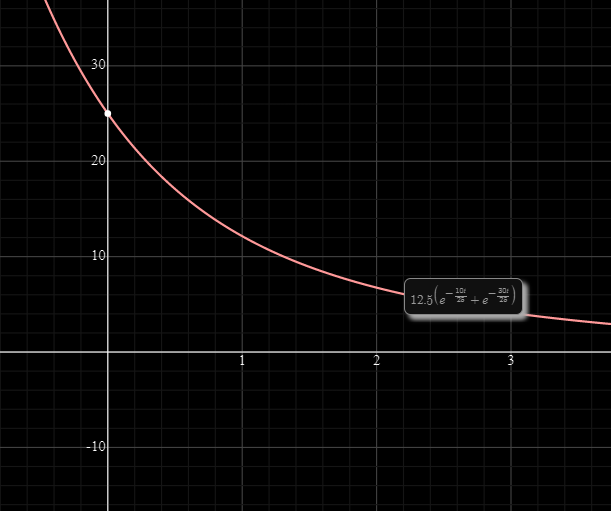
\includegraphics[scale=0.5]{Imagenes/Ejercicio7a.png}\\

\textsc{Tanque B}\\
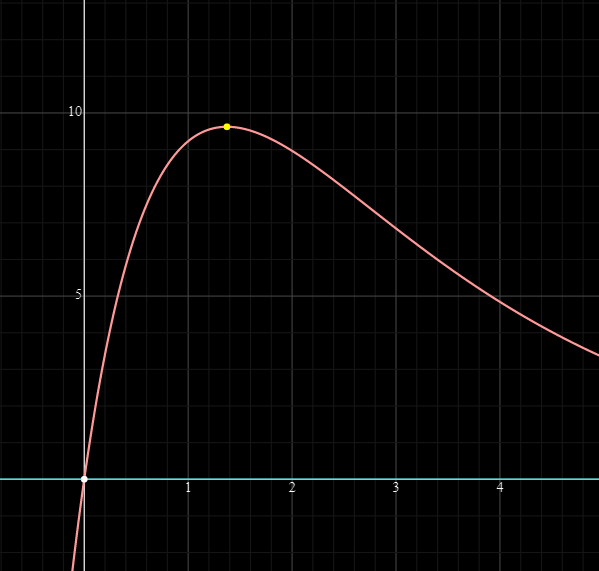
\includegraphics[scale=0.4]{Imagenes/Ejercicio7b.png}
